\chapter{Grundlagen}
In diesem Kapitel werden alle notwendigen Hintergrundinfos zum Verständnis der Arbeit gegeben.

\section{Transformer}
Die Architektur des Transformer Modells wurde erstmals 2017 von Vaswani \textcite{Vaswani2017} vorgestellt und stellt eine fundamentale Neuerung im Bereich der neuronalen Netze und natürlicher Sprachverarbeitung dar (NLP) dar. Die Transformer-Architektur verzichtet vollständig auf rekurrente oder konvolutionale Mechanismen und setzt stattdessen auf einen Selbstaufmerksamkeitmechanismus(Self Attention). Dadurch übertreffen Transformermodelle ältere Modelle wie rekurrente neuronale Netze (RNNs) und Convolutional Neural Networks )CNN) in vielen Anwendungsfällen wie Kontextverständniss, Parallelisierbarkeit und Skalierbarkeit. Darüber hinaus können Transformermodelle universell in verschiedenen Bereichen eingesetzt werden. Die Transformer Architektur bildet die Grundlage für nahezu alle aktuell großen Sprachmodelle wie z.B. BERT, GPT oder T5

In der folgenden Abbildung ist der orignale Aufbau eines Transformermodells schematisch dargestellt

\begin{figure}
\centering
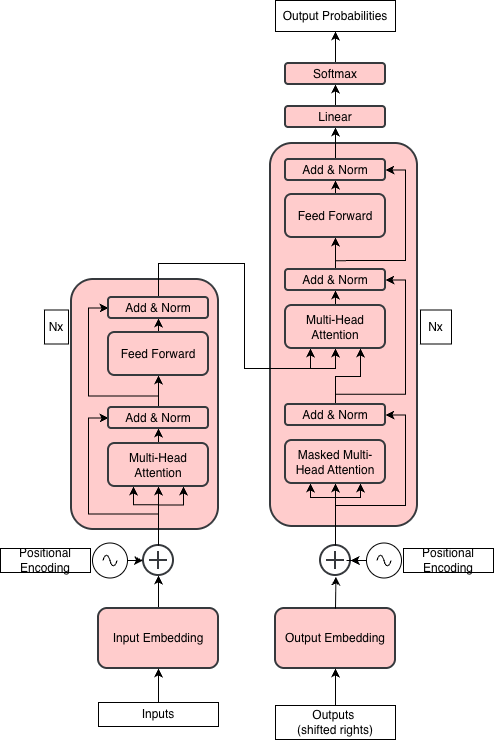
\includegraphics[height=0.7\textheight]{Bilder/encoder_decoder_transformer.drawio.png}
\caption{Decoder-Only Transformer in Anlehnung an  und }
\label{fig:decoder}
\end{figure}

In der originalen, von Vaswani u.a. vorgestellte Transformer Architektur besteht aus Encoder- und Decoderschichten. Der Encoder ist verantwortlich für die Verarbeitung des Eingabetexts und erzeugt daraus eine Reihe kontextualisierter Repräsentationen, welche vom Decoder genutzt werden um Ausgaben, wie einen übersetzten oder vorhergesagten Text, zu generieren. 

Encoder- und Decoderschichten können unabhängig voneinander für Modelle genutzt werden, so hat sich die ursprüngliche Architektur zu drei Architekturrichtungen weiterentwickelt. Encoder-Only (BERT), Decoder-Only(GPT-Modelle) und Encoder-Decoder (T5) eigenen sich für verschiedene Anwendungsgebiete.

Jeder Encoder und Decoder besteht aus weiteren Schichten

Ein zentraler Bestandteil der Transformerarchitektur ist der Selbstaufmerksamkeitsmechanismus (Self-Attention), welcher es ermöglicht kontextuelle Zusammenhänge zwischen den Tokens zu erkennen. Bei diesem werden allen Tokens in der Eingabesequenz Werte je nach relevanz für den Gesamtkontext zugewiesen, wodurch Zusammenhänge über große Distanzen nicht verloren gehen. Die parallele Verarbeitung steigert die Effizienz sowie Qualität der Ausgabe immens, da Tokens nicht sequientiell nacheinander abgearbeitet werden wie bei RNN oder LSTM Modellen.

\begin{itemize}
    \item Self-Attention-Schicht:  
    \item Feed-Forward-Schicht
    \item Residualverbindung und Normalisierung
    
\end{itemize}

1. Self-Attention-Schicht: Berechnung der Beziehung zwischen allen Positionen einer Sequenz
2. Feed-Forward-Schicht: Vearbeitung gewonnener Information
3. Residualverbindung und Normalisierung: Stabilisierung des Trainings und verbessern des Informationsflusses zwischen schichten. 



Besonders GPT 
Generative Pretrained Transformer
Bild mit Aufbau vom Transformer Original und daran beschreiben wie aufgebaut ist 

Vortraining und Finetuning

Anwendungsbereiche für Transformer und bekannte Modelle mit Transformer Architektur
Nachteile im Vergleich zu anderen KI-Modellen 
Darüber hinaus lassen sich Transformer auch für andere Zwecke einsetzten als zur NLP. Transformer werden allerdings nicht ausschließlich für NLP verwendet und finden auch Anwendung in bereichen wie Bildverarbeitung und Audioverarbeitung
-> Whisper als Text to Speech Transformer modell 


\section{Speech-to-Text}
Speech to text bezeichnet die technik um aus gesprochenem inhalt 
Was ist das? Wie funktiniert das? Welche Technik wird hier verwendet? 
Verweis auf Masterprojekt. Wie wurde ausgewähltes Modell feingetuned, bzw wie wird es finegetuned. 
Whisper funktioniert wie ein Transformer, bei dem anstatt wörtern log mel spektogramme ein
Kann ins Detail gehen
Kurz anreißen wie sich technik entwickelt hat, ohne zu sehr ins Detail zu gehen, keine größere Relevanz
Faster Whisper, welches auf Whisper basiert (lediglich inferenz ist anderes) 

Speech-to-Text (STT) auch Automatic Speech Recognition (ASR) beschreibt alle rechnergestützten Verfahren zur automatisierten Umwandlung gesprochener Sprache in schriftliche Form. Ziel ist die robuste Erkennung von Sprache, deren korrekter Interpretation sowie Generierung einer konkreten Textrepräsentation. 

Das Modell Whisper wurde 2022 von OpenAI veröffetnlicht und ist im wesentlichen ein Encoder-Decoder-Transformermodell, welches mit annotierten Audiodaten Trainiert wurde. Dabei verarbeitet der Encoder anstatt Text, Mel-Sektrogramme des Audios mit welchem der Decoder anschließend Text-Tokens verarbeitet. 

Whisper wurde mit etwa 680.000 Stunden multilingualem Audiomaterial trainiert, was es zu einem guten Foundation Modell im Bereich der ASR macht. Durch Finetuning von Whisper lässt sich das Modell darüber hinaus weiter an eigene Bedürfnisse anpassen. 


Encoder: Wandelt das Audiosignal (Mel-Spektogramm) in eine latente Repräsentation um. 

Decoder: Erzeugt auf Basis dieser Repräsentation Text-Token ähnlich wie ein Sprachmodell. 

\section{Large-Language-Model}
Large Language Models (LLMs) sind tiefenlernende neuronale Netze, die auf umfangreichen Sammlungen natürlicher Sprachdaten trainiert werden, um sowohl sprachliches Verständnis als auch generative Fähigkeiten zu entwickeln. Im Gegensatz zu älteren, stärker auf spezifische Aufgaben zugeschnittenen NLP-Modellen entstehen durch das Training auf breit gefächerten Textkorpora allgemeine, domänenübergreifende Sprachfertigkeiten. Daher werden moderne LLMs häufig als Foundation Models bezeichnet, da sie eine vielseitige Grundlage für eine Vielzahl nachgelagerter Anwendungen bieten (Zhao et al., 2023; Minaee et al., 2024).

Technologisch basieren die meisten heutigen LLMs auf der Transformer-Architektur, die durch Mechanismen wie Self-Attention eine effiziente Verarbeitung langer Textsequenzen ermöglicht und damit die zuvor gängigen rekurrenten Modelle weitgehend abgelöst hat. Ein charakteristisches Merkmal von LLMs ist ihre enorme Größe: Sie umfassen häufig Milliarden von Parametern und werden auf Datensätzen im Größenbereich vieler hundert Gigabyte bis hin zu mehreren Terabyte trainiert. Empirische Scaling Laws zeigen, dass mit wachsenden Modellparametern, größeren Datensätzen und höherer Rechenleistung systematisch Leistungssteigerungen erzielt werden können (Zhao et al., 2023).

Der Trainingsprozess moderner LLMs erfolgt in zwei Schritten. Zunächst werden die Modelle im Pre-Training mittels selbstüberwachtem Lernen trainiert. Typische Lernziele sind das Vorhersagen des nächsten Tokens oder das Auffüllen maskierter Textteile. Dieser Prozess führt zu einer breit angelegten, generalistischen Sprachkompetenz. Darauf aufbauend folgt das Fine-Tuning, bei dem ein vortrainiertes Modell durch überwachtes Lernen auf spezifische Aufgaben oder Daten angepasst wird. Fine-Tuning kann das gesamte neuronale Netz betreffen, jedoch haben sich in den letzten Jahren auch parameter-effiziente Methoden wie LoRA (Low-Rank Adaptation) etabliert. Bei LoRA werden nur kleine, trainierbare Zusatzmatrizen ergänzt, während der Großteil der ursprünglichen Modellparameter eingefroren bleibt. Dies reduziert den Rechenaufwand erheblich und ermöglicht die Anpassung großer Modelle auf vergleichsweise kleinen Datensätzen.

Ein weiteres Schlüsselmerkmal aktueller LLMs ist ihre Fähigkeit zu In-Context Learning. Das Modell nutzt dabei allein auf Basis der im Prompt bereitgestellten Beispiele oder Instruktionen neue Aufgabenstrukturen, ohne dass Parameteränderungen notwendig sind. Damit entsteht eine bemerkenswerte Flexibilität: Das Modell kann Aufgaben lösen, für die es nie explizit trainiert wurde, sofern die Aufgabenbeschreibung im Kontext ausreichend präzise ist.

Die Entwicklung von LLMs markiert einen Paradigmenwechsel in der Sprachverarbeitung. Während klassische Sprachmodelle primär die Wahrscheinlichkeit des nächsten Tokens schätzten, generieren heutige Modelle konsistente, kontextbezogene Texte, beantworten Fragen, strukturieren Inhalte und zeigen zunehmend komplexes reasoning-ähnliches Verhalten. Dadurch verschiebt sich der Fokus von reiner Sprachmodellierung hin zu einer generativen, vielseitig einsetzbaren Sprachintelligenz (Minaee et al., 2024).


\section{NLP mit Hilfe von KI}
Bei der verarbeitung von Sprache und Text mithilfe von KI gibt es verschiedene Methoden. Zum verständnis dieser Arbeit werden nicht alle gezeigt. 
Extractive und abstractive Summary 

\subsection{Segmentation}
Zerteilung von Texten in kleinere, verarbeitbare Einheiten (Segmente) bevor LLM den Inhalt analysiert oder Zusammenfasst

Modelle haben nur begrenzte Kontextlänge (Tokens), wird die Kontextlänge überschritten, kann das Modell den Inhalt nicht komplett verarbeiten



Text wird in logisch sinnvolle einheiten aufgeteilt, Absätze, Kapitel, Themenblöcke
Fixed Size Segmentation: Text wird nach einer Bestimmten Tokenzahl geteilt, recht einfach, geht aber nicht auf Textinhalte ein. Cut eventuell direkt im Kapitel 
Semantic segmentation: Text wird mit inhaltlichen Grenzen getrennt. Oft mithilfe von Embeddings oder Clustering

Embedding: Umwandlung von Wörtern und Text in Vektoren, Vektoren mit ähnlichem Embedding sind Inhaltlich näher beieinander als Vektoren mit großem Abstand im Embedding 

Clustering: Mehrere Embeddings die sich Ähneln werden zu einem Cluster zusammengefasst -> Semantisch homogene Segmente. 

-> Text lässt sich somit mit inhaltlichen Grenzen trennen


Hybrid Ansatz, Kombination aus beidem 

\subsection{Kontextualisierung}
Fähigkeit des LLMS den Sinn eines Textes im Größeren Zusammenhang zu erfassen. 
Wichtigkeit einzelner Bereiche wird durch Kontextualisierung hervorgehoben.
Gesamtzusammenhang wird erkannt und berücksichtigt bei der Verarbeitung

Kontext gezielt zu nutzen ist entscheidend für die Qualität, Faktentreue und Kohärenz bei LLMs und langen Dokumenten (On Context Utilization in Summarization with large language Models) 

LLMs bei langen Eingaben oft nur Teile des Inputs effektiv nutzen, insbesondere den Anfang und das Ende. Inhalte in der Mitte bleiben unterräpresentiert (Positionsbias) 
(On Context Utilization in Summarization with Large Language Models)

-Wichtige Querverweise, temporale Bezüge oder Implikationen bleiben unterberücksichtigt. 

Bei Sprache zu Text spielt kontextualisierung besonders große Rolle, da es bei Transkripten oftmals Sprecherwechsel, Themenwechsel und referentielle Sprünge gibt. 

Es wird zwischen verschiedenen Arten der Kontextualisierung unterschieden: 
1. Intra-Dokument Kontext: Bezieht sich auf Zusammenhänge innerhalb eines Dokuments oder Textsequenz. Durch einbindung des Globalen Kontext lassen sich bessere Zusammenfassungen erstellen, im vergleich zur ausschließlichen Lokalen Satzbereiches 
(Contextualized Rewriting for Text Summarization) 

2. Inter Dokumentärer oder externer Kontext: 
Dabei werden 

3. Simulatane Berücksichtigung von Struktur- und Sprecherwechseln 
Bei Gesprächs- oder Transkript-Daten wie bei der Verwendung von Speech to Text Modellen wie Whisper spielt es eine Rolle, dass da Modell versteht, wer spricht, wie Themen wechseln und Referenzen verlaufen. 
(Context aware hierarchical attention for abstractive dialogue summarization)



\subsection{Rolling Summary}
Was ist das? Wie Funktioniert ds und wie lässt sich das 
Mehrstufige Zusammenfassung, Text wird nicht in eins zusammengefasst sondern vorher in chunks/Teilstücke aufgeteilt, welche einzeln zusammengefasst werden. Text wird schrittweise verdichtet

Eignet sich gut bei Texten oder Daten, welche in vielen kleinen Segmenten vorliegt. (Chatverläufe, Dokumentensammlung oder Meeting Transkripte)

1. Text wird in Chunks aufgeteilt, 
2. Chunks werden einzeln zusammengefasst 
3. Teilzusammenfassungen werden anschließend wieder zusammengefasst 
4. Finale verdichtung: Es entsteht eine kompakte Gesamtzusammenfassung, welche die wichtigsten Kernaussagen aller Teile enthält. 

Incremental rollup summarization

Beispielbild 

Vorteile: Skalierbarkeit, Speichereffizienz 
Nachteile: möglicher Informationsverlust, Bias Kaskade (Fehler oder Gewichtungen aus unteren Stufen ziehen sich bis nach oben) 

Balancierung, Wie stark soll jeder Chunk zusammengefasst werden? Oberflächlichkeit vs Redundanz 


\section{Prompt Engineering}
Was das und wie wird es hier mit eingebracth? 
Verschiedene Arten von Prompts: 
-Benutzerprompt -> Anweisungen vom Benutzer
-Systemprompt -> Instruktionen für bestimmte KI-Agenten, wird dem Nutzer nicht angezeigt
-Agentenprompt -> Ausgabe des KI-Agenten

Gezielte Gestalten von Eingabeaufforderungen ("Prompts") für Large Language Modelle um gewünschte Ausgabe zu erzielen ohne Modellparameter zu verändern. (A Systematic Survey of Prompt Engineering in Large Language Models: Techniques and Applications)
Prompts können in verchiedenen Formen auftreten wie natürlicher sprache, Beispielen oder als soft Prompts in Vektorrepräsentation vorliegen. 

Ziel: Mithilfe von geschicktem Prompt engineering beretis vortrainierte Modelle auf spezifische Aufgaben anzusetzen ohne Feintuning großer Parameter (Unleashing the potential of prompt engineering for large language models)

Prompt Engineering spart zeit, da umfangreiches Feintuning reduziert werden kann oder ganz wegfällt. Vorhandene Kapazität des LLMs wird durch geschickte Eingaben genutzt. 

Zero-Shot-Prompting: Modell erhält nur eine Aufgabenstellung ohne Beispiele
Few Shot Prompting: Modell erhält wenige Beispielpaare (Input-Output) um sich zu Orientieren
Chain-of-Thought (Cot) Prompting: 

Qualität des Prompts hängt stark von Formulierung, Klarheit, Kontext und Beispielwahl ab. Unterschiedliche formulierungen können zu sehr unterschiedlichen resultaten Liefern (The Prompt Report: A Systematic Survey of Prompt Engineering Techniques)
Prompts sind Modellspezifisch, ein prompt der bei modell a gut funktioniert muss nicht bei modell b funktionieren 
Evaluation schwierig: Es existieren noch nicht immers tandardisierte Metriken. Wie wird ein "guter" Prompt gemessen. (Sehr Subjektiv)
(A Systematic Survey of Prompt Engineering in Large Language Models: Techniques and Applications) 

"Mehr ist nicht immer besser" -> Mehr Beispiele oder Längerer Kontext führt nicht automatisch zu besseren Ergebnissen. Effekte von Übertransfer oder Ablenkung 

(A Systematic Survey of Prompt Engineering in Large Language Models: Techniques and Applications) - Gibt eine Liste mit vielen Techniken für LLMs an 



\section{Weitere Hilfsmittel und Tools}
\subsection{RAG}


